\documentclass[a4paper,11pt]{article}
\usepackage{latexsym}
\usepackage[italian]{babel}
\usepackage[utf8]{inputenc}  
\usepackage{pdfsync}
\usepackage{moreverb}
\usepackage{listings}
\usepackage{graphicx}
\author{Alessio Caiazza, Cosimo Cecchi}
\title{CaptureMJPEG: a MotionJPEG library for Procesing}
\frenchspacing
\begin{document}
\maketitle

\newcommand{\reffigura}[1]{
  Figura \ref{#1}
}

\begin{abstract}
CaptureMJPEG è una libreria per
Processing\footnote{http://processing.org} che consente di gestire uno
stream motion-jpeg come input video.\\
La libreria è in grado di acquisire lo stream tramite i protocolli
\mbox{HTTP/HTTPS} e dispone di alcune classi di aiuto per la generazione di
URL per le videocamere di rete AXIS e Sony.  
\end{abstract}
\tableofcontents


\section{Introduzione}
\label{sec:introduzione}
%Cosa è stato fatto, come e con quali obiettivi
%Presentazione del progetto e del sito
All'inizio dello sviluppo di CaptureMJPEG ci siamo chiesti quali
fossero le linee guida da seguire. Ci siamo trovati d'accordo sul
fatto che la libreria fosse rivolta ad una base di utenza non
avanzata, composta da grafici o programmatori alle prime armi. Abbiamo
optato quindi per una soluzione che privilegiasse la facilit\`a d'uso
rispetto alla complessit\`a e alla ricchezza dell'API offerta,
rimanendo in linea con la filosofia di Processing.\\
Un esempio di questa scelta si pu\`o rintracciare nella gestione delle
eccezioni, trasparente all'utente grazie alla rappresentazione di esse
tramite immagini, quindi usabili senza alcun codice aggiuntivo di
correzione dell'errore.\\
Per facilitare l'apprendimento, una particolare attenzione \`e stata
posta nel rispettare le convenzioni delle librerie del core di
Processing, prendendo esempio dal comportamento della classe
\texttt{Capture}.\\
Per lo sviluppo, ci siamo avvalsi di strumenti open-source per la
gestione del versionamento e per la creazione di un sito del progetto
che fosse allo stesso tempo facile da consultare per gli utenti ma
anche ricco di funzionalit\`a rivolte agli sviluppatori. Da questa
esigenza \`e nata la scelta di Trac come motore per il sito del
progetto. Il VCS che abbiamo scelto per lo sviluppo \`e Mercurial, per
la facilit\`a di integrazione con Trac e per la possibilit\`a di
effettuare commit e visionare il log del progetto anche offline. Il
codice \`e stato sviluppato con Eclipse, grazie al quale abbiamo avuto
la possibilit\`a di sperimentare una programmazione task-oriented,
grazie all'utilizzo integrato di Mylyn.\\
Si \`e scelto infine di utilizzare la tecnica del peer-programming per
lo sviluppo, che consiste nello scambiarsi nel ruolo di scrittura e
revisione del codice, minimizzando gli errori dovuti a stanchezza e
distrazione e il tempo necessario alla revisione del codice e
all'apprendimento di gruppo.

\section{Manuale}
\label{sec:manuale}
Guida all'installazione ed utilizzo di CaptureMJPEG
\subsection{Installazione}
\label{sec:installazione}
%scopiazzare dal sito e tradurre in italiano
Per prima cosa scaricare l'ultima versione di CaptureMJPG dal sito
ufficiale http://capturemjpeg.lilik.it .\\
Una volta ottenuto l'archivio decomprimerlo all'interno della
sottocartella \texttt{contributed} del proprio sketchbook, su Linux
solitamente è \texttt{$\sim$/sketchbook}, su Mac OS X e Windows
è la cartella \texttt{Processing} all'interno dei propri documenti.\\
Qualora la sottocartella \texttt{contributed} non esistesse è
necessario crearla.\\
A questo punto riavviare Processing. 
\subsection{Guida all'utilizzo}
\label{sec:guida}
%inserire un po' di esempi e spiegare le funzioni utilizzabili
La libreria si trova nel package \texttt{it.lilik.capturemjpeg}.\\
La classe fondamentale \`e \texttt{CaptureMJPEG}, che dispone dei metodi
necessari per la gestione dello stream e per l'integrazione con processing.
Per una documentazione completa sulle classi offerte dal package e i relativi
metodi disponibili si rimanda alla documentazione JavaDoc sul sito del 
progetto.\footnote{http://capturemjpeg.lilik.it/doc/}\\

Per ottenere un oggetto di tipo \texttt{CaptureMJPEG} \`e necessario invocare
il suo costruttore con l'URI della videocamera come parametro. Per questa
finalit\`a, la libreria mette a disposizione delle classi per creare facilmente
gli URI a partire dalla marca della videocamera, correntemente sono
implementate solo quelle per le videocamere Sony e AXIS.\\
Una volta ottenuto l'oggetto \texttt{CaptureMJPEG} abbiamo a disposizione due
modalit\`a per gestire lo stream proveniente dalla videocamera. La prima,
chiamata modalit\`a di callback, prevede la definizione di un metodo
all'interno dello sketch, che verr\`a invocato dalla libreria ogni volta che
un nuovo fotogramma \`e pronto. La modalit\`a senza callback, invece, prevede
che i fotogrammi siano salvati, non appena disponibili, in un buffer circolare
interno alla libreria e accessibile tramite il metodo \texttt{getImage ()}.\\
Un programmatore che usa la libreria ha la garanzia che il flusso restituito
sar\`a sempre costituito da immagini. Infatti gli eventuali errori sono gestiti
internamente alla libreria, che provveder\`a a creare delle immagini con una
descrizione testuale dell'errore in caso di problemi.
\subsubsection{Esempi}
\label{sec:utilizzo_esempi}
Qui di seguito sono illustrati vari esempi di utilizzo della libreria.\\

L'esempio in \reffigura{fig:basic_usage} illustra l'utilizzo di base di CaptureMJPEG.
Si nota la funzione di callback \texttt{captureMJPEGEvent}, invocata dalla libreria quando
sono disonibili nuovi frame. In questo esempio \`e utilizzato il parser di
default per gli URI. Si noti che in questo caso \`e necessario specificare
l'URI completo di protocollo.\\

Il secondo esempio in \reffigura{fig:vendor_specific} illustra la modalit\`a
d'uso dei costruttori di URI specializzati. In questo caso \`e necessario
inserire solamente l'host come parametro del costruttore dell'URI.\\

Il terzo esempio in \reffigura{fig:buffer_usage} illustra l'utilizzo del buffer
interno alla libreria. Si noti l'utilizzo del metodo \texttt{getImage ()} per
ottenere il fotogramma successivo dello stream.\\

Infine, l'esempio in \reffigura{fig:adaptive_fsize} mostra come sia possibile
far s\`i che la dimensione dell'applet si adatti alla dimensione dello stream,
attraverso la chiamata al metodo \texttt{setAdaptiveFrameSize ()}.\\

\section{Analisi}
\label{sec:analisi}

\subsection{Comparazione dell'algoritmo blur fra CaptureMJPEG e Capture}
\label{sec:comparazione}

%Studio della libreria eseguito con il codice di prova
L'analisi è stata svolta applicando un filtro \texttt{blur} allo
stream ottenuto con CaptureMJPEG e con la videocamera locale
utilizzando la libreria Capture\footnote{la libreria Capture è fornita
  in bundle con Processing.}.\\
I sorgenti utilizzati sono quelli in \reffigura{fig:micc_blur} per
CaptureMJPEG e in \reffigura{fig:capture_blur} per Capture.
Sono stati misurati l'utilizzo di memoria e di CPU al variare delle
dimensioni del filmato e del framerate richiesto allo sketch.\\
L'analisi ha riportato un utilizzo di memoria minore per la libreria
CaptureMJPEG, 30MB contro 40MB per il filmato a risoluzione 320x240 e
50MB contro 60MB per il filmato a risoluzione 640x480.\\

L'utilizzo di CPU è riportato in \reffigura{fig:blur_isto}.
L'algoritmo applicato allo stream di risoluzione 320x240 mostra un
utilizzo di CPU più pesante da parte di CaptureMJPEG in media del
11.7\% mentre con lo stream a risoluzione 640x480 l'utilizzo è più
pesante da parte della libreria Capture, con un distacco fisso del
5\%.\\
Si deve considerare inoltre il fatto che CaptureMJPEG utilizza
connessioni HTTP remote mentre Capture utilizza il bus USB ad alta
velocità del sistema locale.\\

I test sono stati eseguiti su un iMac con la seguente configurazione:
\begin{tabbing}
  \textbf{sistema operativo} \= Mac OS X 10.4.11 \kill

  \textbf{processore} \>Intel Core Duo 2GHz (32 bit, dual core)\\
  \textbf{memoria RAM} \> 1GB a 667MHz \\
  \textbf{sistema operativo} \> Mac OS X 10.4.11 \\
  \textbf{processing} \> 0135 beta \\
\end{tabbing}


\subsection{Impressioni qualitative}
\label{sec:impressioni}
Dall'osservazione del comportamento della libreria nei test effettuati,
si evince che la modalit\`a di callback ha un comportamento ottimale per la
realizzazione di sketch con fine di monitoraggio o di visione delle immagini,
dato che tutti i frame provenienti dalla videocamera sono resi disponibili
al programmatore. Se invece si vuole applicare trasformazioni alle immagini,
mantenendo la sincronia con il flusso proveniente dalla videocamera, allora
si consiglia l'uso della modalit\`a senza callback, dato che gli eventuali
frame non estratti dal buffer, perch\'e impegnati in operazioni di processing,
sono automaticamente scartati dal sistema.

\section{Sviluppo}
\label{sec:sviluppo}
Come continuare lo sviluppo
\subsection{Ottenere i sorgenti}
\label{sec:sorgenti}
Prima di scaricare i sorgenti è necessario installare
Mercurial\footnote{Mercurial può essere scaricato dal sito
 http://www.selenic.com/mercurial/}, 
per la gestione dei sorgenti ed Ant\footnote{Ant può essere scaricato
dal sito http://ant.apache.org}, 
per la gestione della compilazione.

Per ottenere i sorgenti eseguire la clonazione del repository
mercurial disponibile all'indirizzo
\texttt{http://dev.abisso.org/capturemjpeg} 
dopodiché creare una copia del file \texttt{user\_pref.xml.template}
con nome \texttt{user\_pref.xml}.

Il file contiene la configurazione di ant per il progetto, tutti i
valori di default vanno bene ad eccezione della ``property''
\texttt{processing-core} che deve essere corretta con la path completa
al file \texttt{core.jar} incluso nella propria installazione di Processing.
\begin{verbatim}
<property name="processing-core" 
    value="C:\Programmi\processing-0135-expert\lib\core.jar" />
\end{verbatim}

A questo punto è necessario eseguire il dowload delle librerie incluse
in CaptureMJPEG eseguendo il comando:
\begin{verbatim}
   ant download_deps
\end{verbatim}

Quindi è possibile generare l'intera cartella di installazione con
il comando:
\begin{verbatim}
   ant deploy 
\end{verbatim}
\begin{figure}
  \centering
\begin{boxedverbatim}

 hg clone http://dev.abisso.org/capturemjpeg capturemjpeg   
 cd capturemjpeg
 cp user_pref.xml.template user_pref.xml

\end{boxedverbatim}
\\
\vspace{0.3cm}
Esempio: ottenere i sorgenti da terminale
\end{figure}

\subsection{Classi utilizzate}
\label{sec:classi}
Forniamo ora una descrizione sommaria delle classi sviluppate per la
libreria, per una trattazione più approfondita si rimanda alla
documentazione JavaDoc disponibile online all'indirizzo 
http://capturemjpeg.lilik.it/doc/.
In \reffigura{fig:class_diagram1} e in \reffigura{fig:class_diagram2}
si pu\`o visualizzare il diagramma delle classi della libreria.\\
Il metodo con cui vengono acquisite le immagini dalla videocamera \`e basato
sull'identificazione all'interno dello stream HTTP proveniente da essa,
dell'elemento che separa le singole immagini, ovvero il \texttt{boundary}.
La prima operazione eseguita all'inizializzazione della libreria \`e dunque 
l'instaurazione di una connessione HTTP al server specificato, tramite le
classi \texttt{HTTPClient} di Apache. Una volta ottenuta la connessione,
l'operazione seguente \`e l'identificazione del boundary, che pu\`o variare
a seconda della marca e del modello della videocamera a cui siamo connessi.
Il boundary \`e comunque specificato nell'header della risposta HTTP della
videocamera, all'interno del campo \texttt{Content-Type}. Questo compito
\`e svolto dalla classe \texttt{CaptureMJPEG}, che implementa quanto illustrato
tramite un thread.\\
Una volta ottenuto il boundary, le immagini sono estratte dallo stream tramite
un meccanismo basato sulla rilevazione dell'identificativo di mime-type
proprio delle immagini JPEG. A tal proposito, abbiamo ritenuto
oppurtuno implementare una classe, \texttt{MJPEGInputStream}, che ereditasse
dalla classe \texttt{java.io.FilteredInputStream} e che ha il suo metodo
fondamentale in \texttt{byte[] readImage ()}, che restituisce un array
contenente l'immagine in formato JPEG.\\
Dopo l'acquisizione di un'immagine, il codice valuta se sia presente o meno
il meccanismo di callback e in caso negativo, l'immagine ottenuta viene salvata
in un buffer circolare, implementato in \texttt{CircularBuffer}.\\
La classe \texttt{ErrorImage} si occupa di generare immagini rappresentanti
un'eventuale errore nel processo, mentre le classi \texttt{AxisURL} e 
\texttt{SonyURL} hanno il compito di costruire un URL a partire dai parametri
specifici supportati dalle videocamere della relativa marca.

\begin{figure}
  \centering
\lstinputlisting[language=Java,numbers=left,frame=shadowbox]{sources/basic_usage.pde}
  \caption{Esempio di utilizzo base}
  \label{fig:basic_usage}
\end{figure}
\begin{figure}
  \centering
\lstinputlisting[language=Java,numbers=left,frame=shadowbox]{sources/vendor_specific.pde}
  \caption{Utilizzo dei costruttori specializzati}
  \label{fig:vendor_specific}
\end{figure}
\begin{figure}
  \centering
\lstinputlisting[language=Java,numbers=left,frame=shadowbox]{sources/buffer_usage.pde}
  \caption{Esempio dell'utilizzo del buffer}
  \label{fig:buffer_usage}
\end{figure}
\begin{figure}
  \centering
\lstinputlisting[language=Java,numbers=left,frame=shadowbox]{sources/adaptive_fsize.pde}
  \caption{Utilizzo della dimensione adattiva}
  \label{fig:adaptive_fsize}
\end{figure}
\begin{figure}
  \centering
\lstinputlisting[language=Java,numbers=left,frame=shadowbox]{sources/micc_blur.pde}  
  \caption{Sorgente di test CaptureMJPEG}
  \label{fig:micc_blur}
\end{figure}
\begin{figure}
  \centering
  \lstinputlisting[language=Java,numbers=left,frame=shadowbox]{sources/capture_blur.pde}
  \caption{Sorgente di test Capture}
  \label{fig:capture_blur}
\end{figure}

\begin{figure}
  \centering
  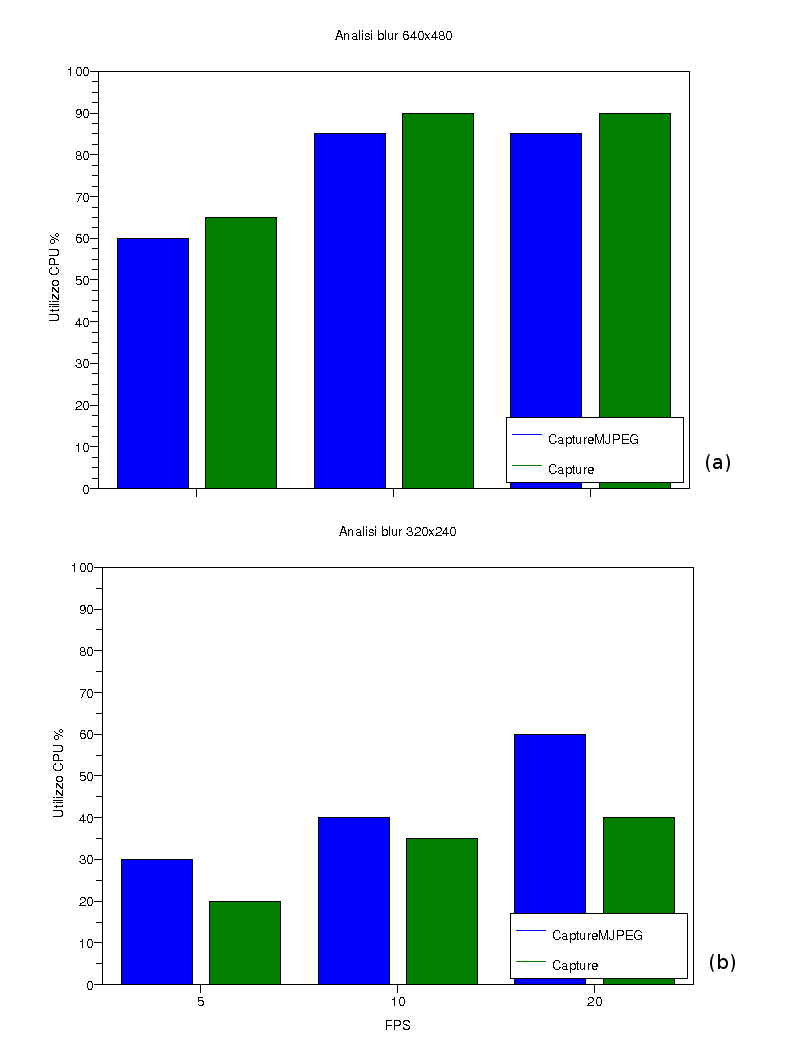
\includegraphics[scale=2.0]{img/istogrammi.png}
  \caption{Analisi algoritmo blur}
  \label{fig:blur_isto}
\end{figure}
% \begin{figure}
%   \centering
%   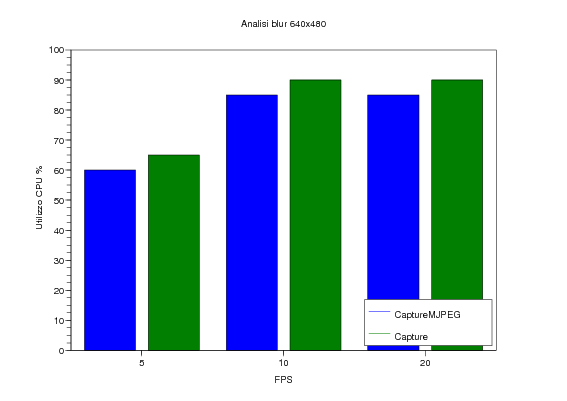
\includegraphics[scale=0.9]{scilab/isto_blur_640.png}
%   \caption{Analisi algoritmo blur 640x480}
%   \label{fig:blur_640}
% \end{figure}
% \begin{figure}
%   \centering
%   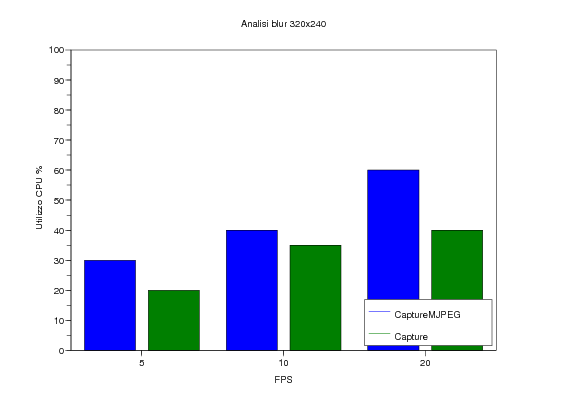
\includegraphics[scale=0.9]{scilab/isto_blur_320.png}
%   \caption{Analisi algoritmo blur 320x240}
%   \label{fig:blur_320}
% \end{figure}

\begin{figure}
  \centering
  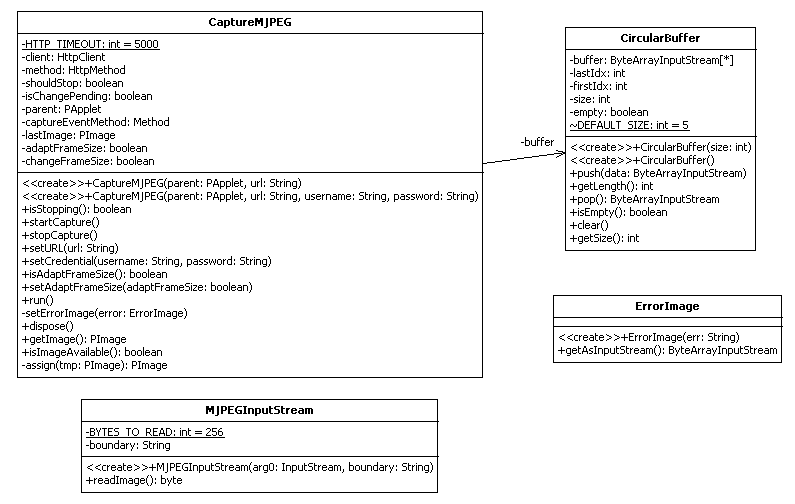
\includegraphics[scale=0.7,angle=90]{img/capturemjpegclass.png}
  \caption{Diagramma delle classi di CaptureMJPEG}
  \label{fig:class_diagram1}
\end{figure}
\begin{figure}
  \centering
  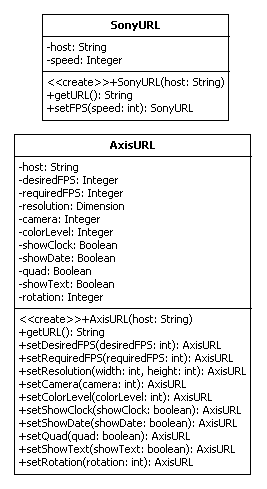
\includegraphics[scale=0.9]{img/uribuilders.png}
  \caption{Diagramma delle classi dei costruttori di URI}
  \label{fig:class_diagram2}
\end{figure}


\end{document}
